\chapter{Үр дүн}

Дээрх хэрэгжүүлэлтийн үр дүнд дараах зургуудад харагдаж байгаачлан манай веб апп маань ашиглахад бэлэн болсон. Доор гол гэсэн хуудсуудын ажиллаж буй процессыг илэрхийлэх хуудсуудын зургуудуудыг оруулав.


Хэрэглэгч рендер хийхэд харагдах хамгийн эхний нүүр хуудас
\begin{figure}[h]
	\centering
	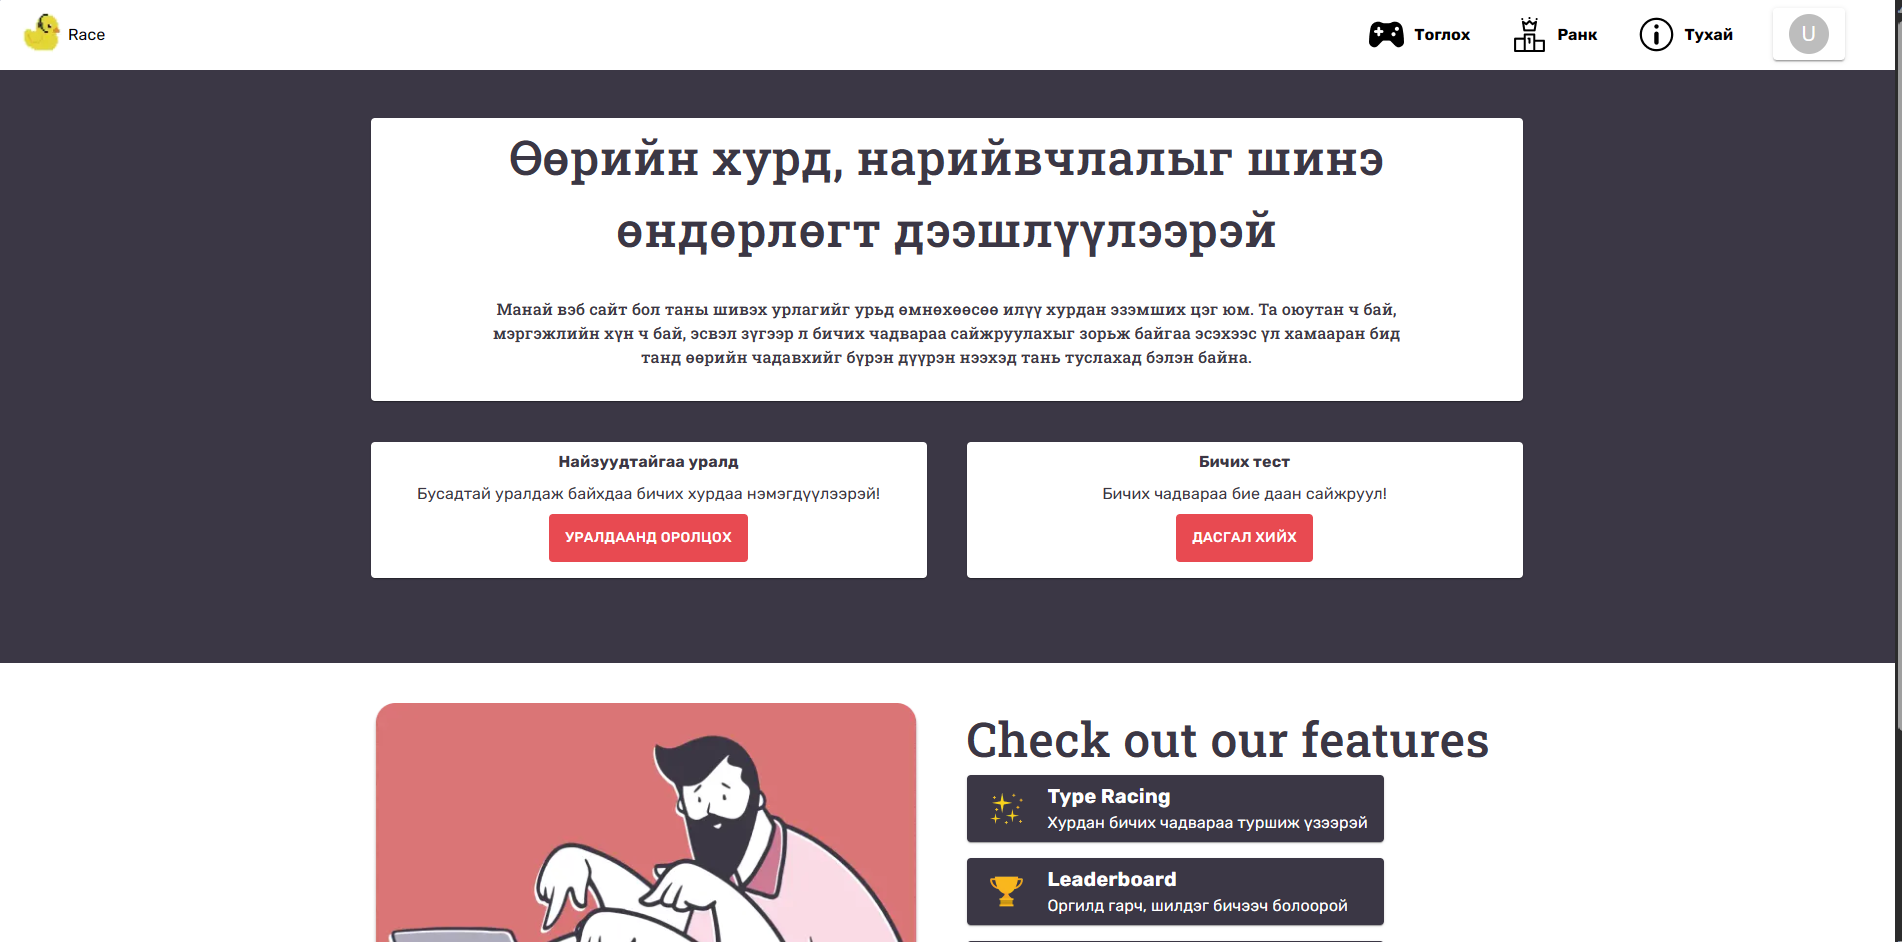
\includegraphics[width=13cm]{images/result/homepage.png}
	\caption{Нүүр хуудас}
	\label{fig:results}
\end{figure}

Singleplayer буюу зөвхөн өөрөө тест өгөх хуудас
\begin{figure}[h]
	\centering
	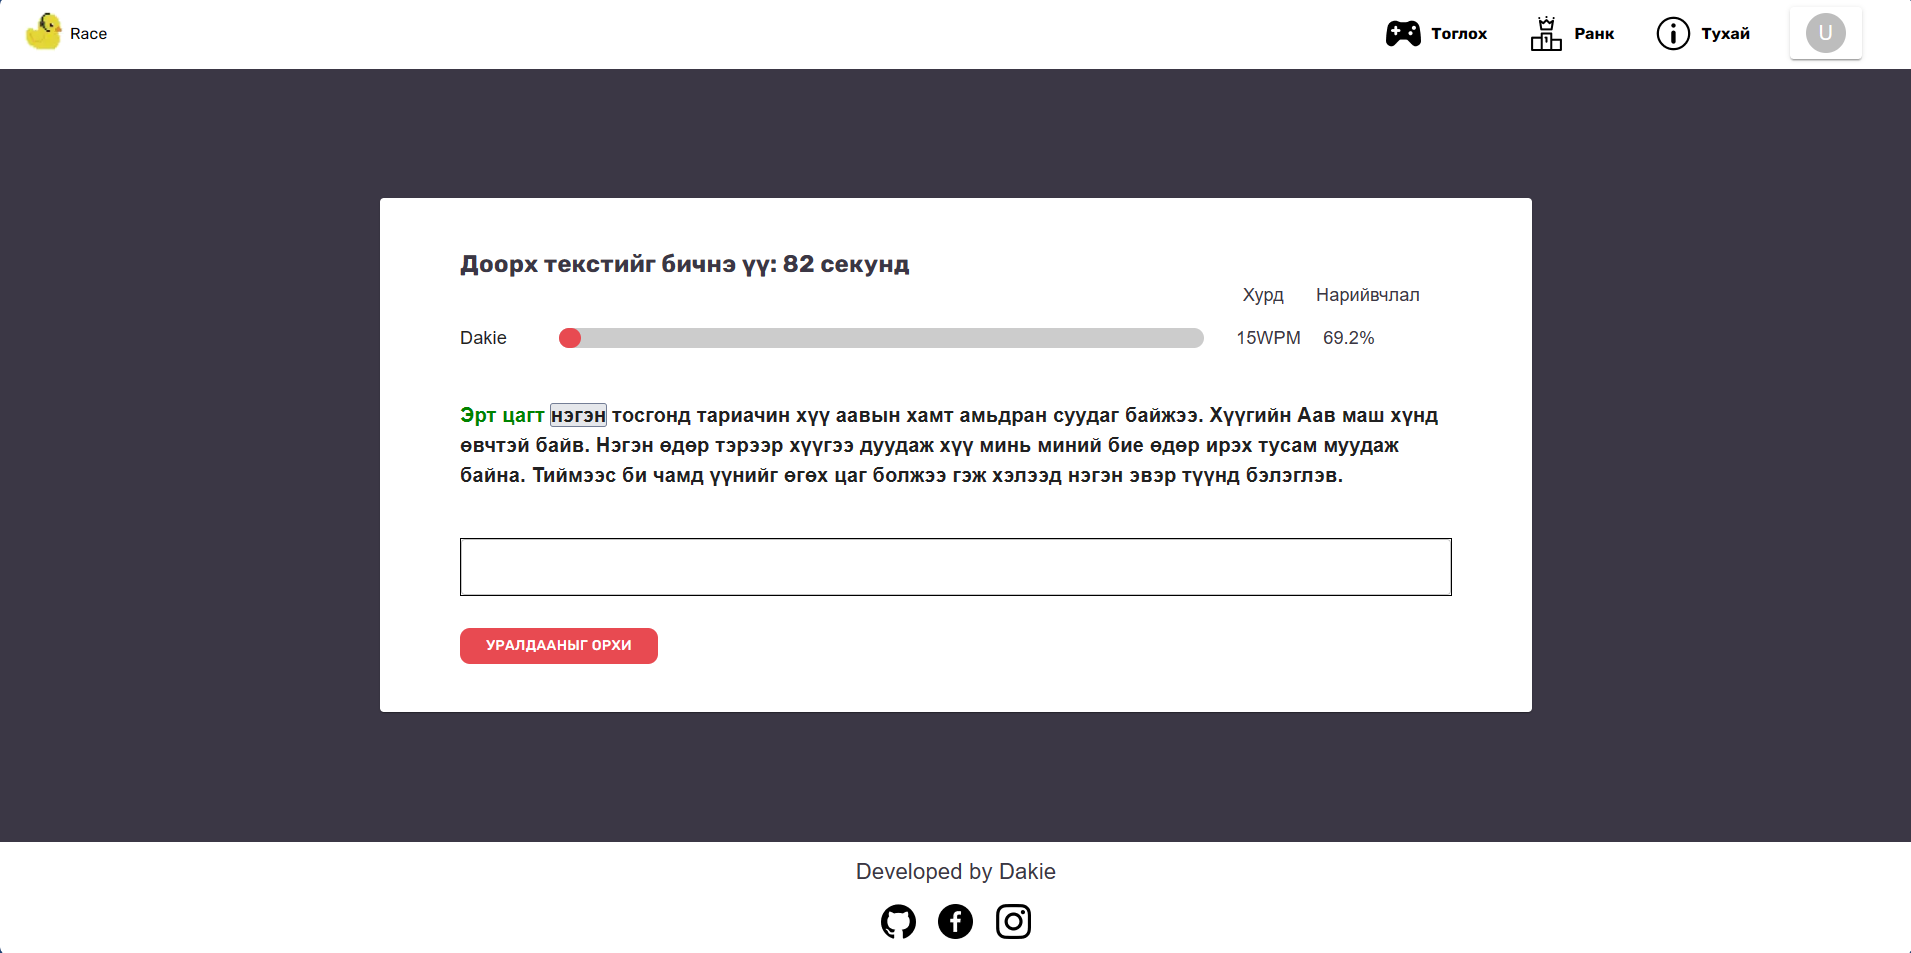
\includegraphics[width=13cm]{images/result/playpage.png}
	\caption{Хэрэглэгч шивэх тест өгөх хуудас}
	\label{fig:results}
\end{figure}

Нийт хэрэглэгчдийг үзүүлэлтээр нь эрэмбэлж харуулах хуудас
\begin{figure}[h]
	\centering
	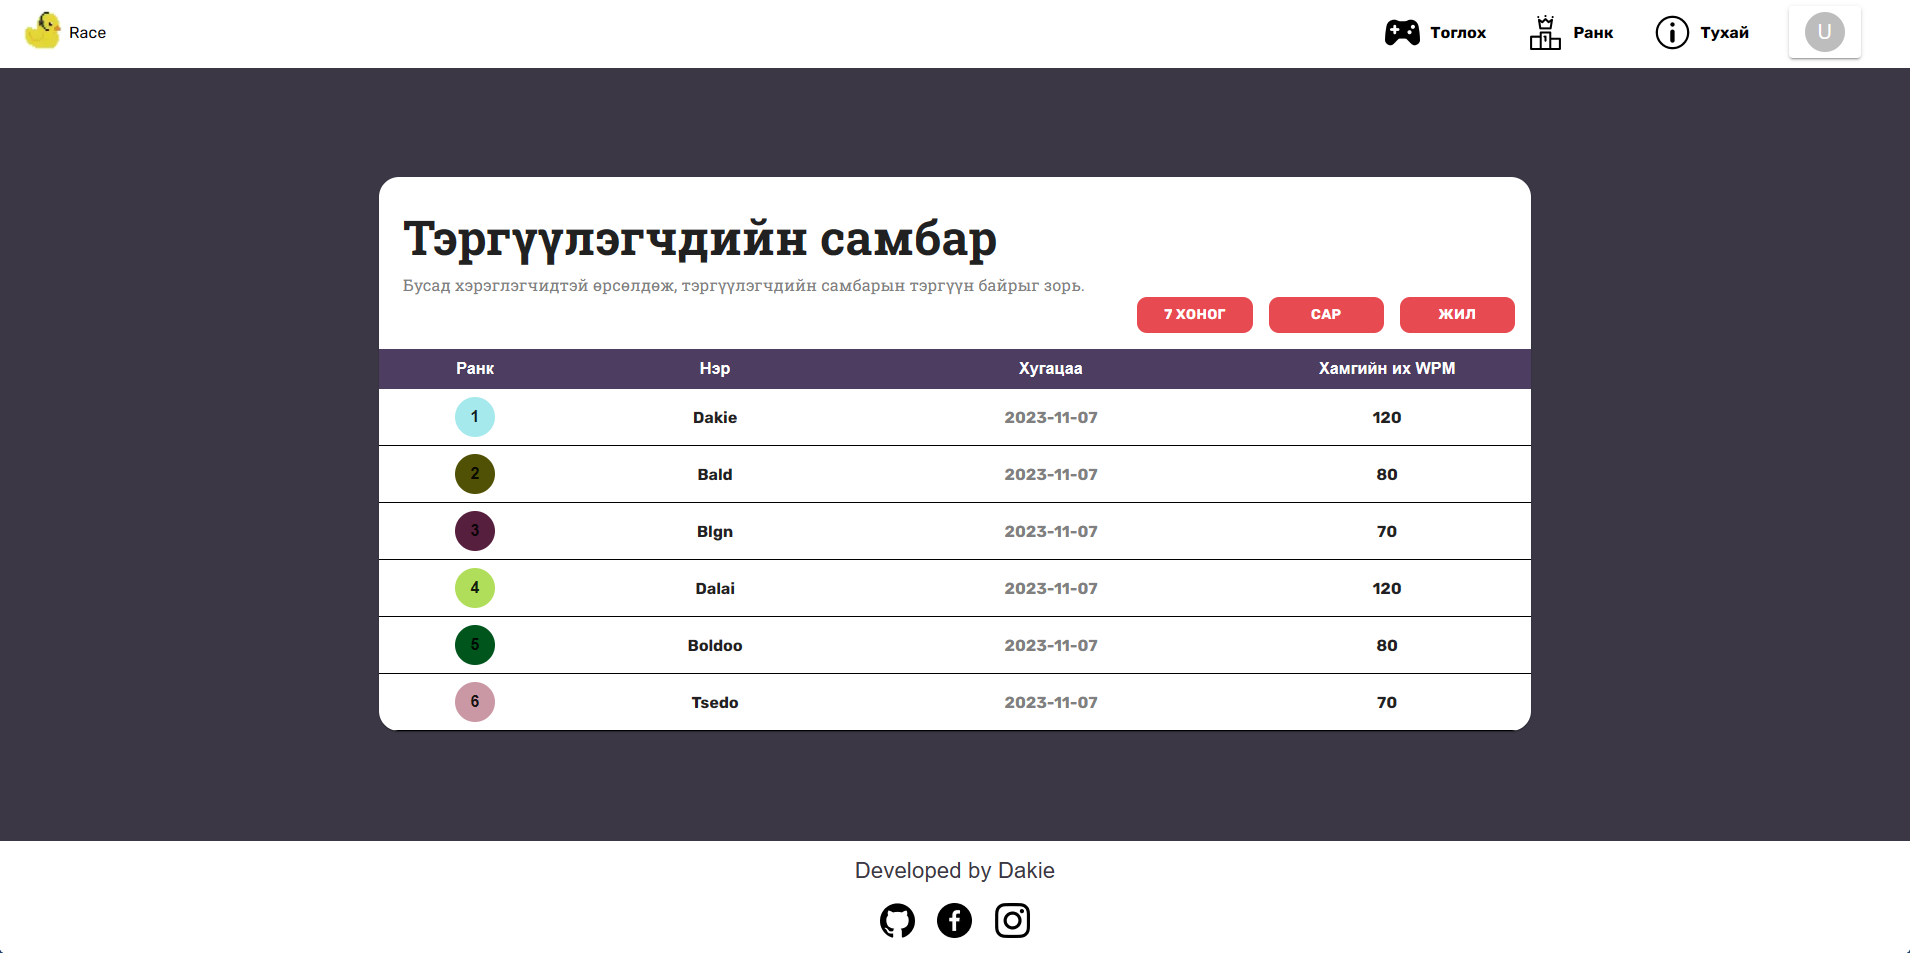
\includegraphics[width=13cm]{images/result/rankpage.png}
	\caption{Нийт тоглогчдыг тэргүүлэгчдийн хуудас}
	\label{fig:results}
\end{figure}

Хэрэглэгч өөрийн үзүүлэлтүүдийг харах хуудас
\begin{figure}[h]
	\centering
	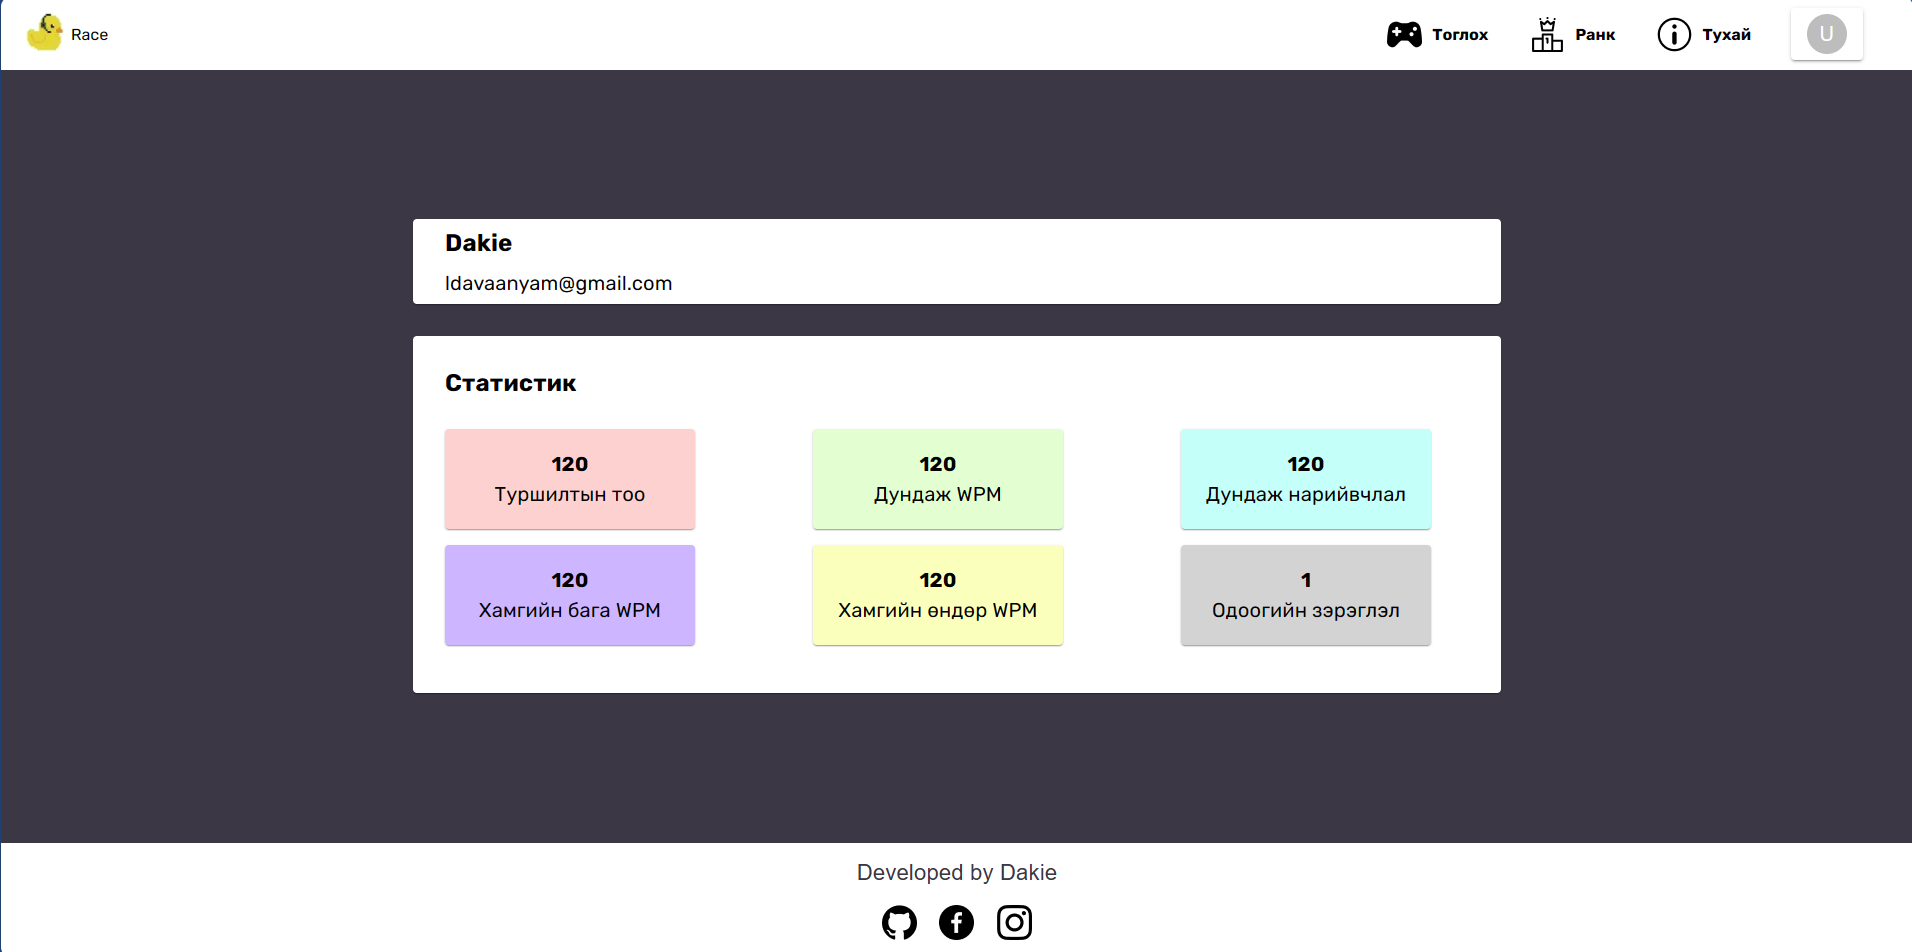
\includegraphics[width=13cm]{images/result/statisticspage.png}
	\caption{Хэрэглэгчийн статистикийн хуудас}
	\label{fig:results}
\end{figure}

Хэрэв хэрэглэгч нэвтрээгүй тохиолдолд рендер хийгдэх хуудас
\begin{figure}[h]
	\centering
	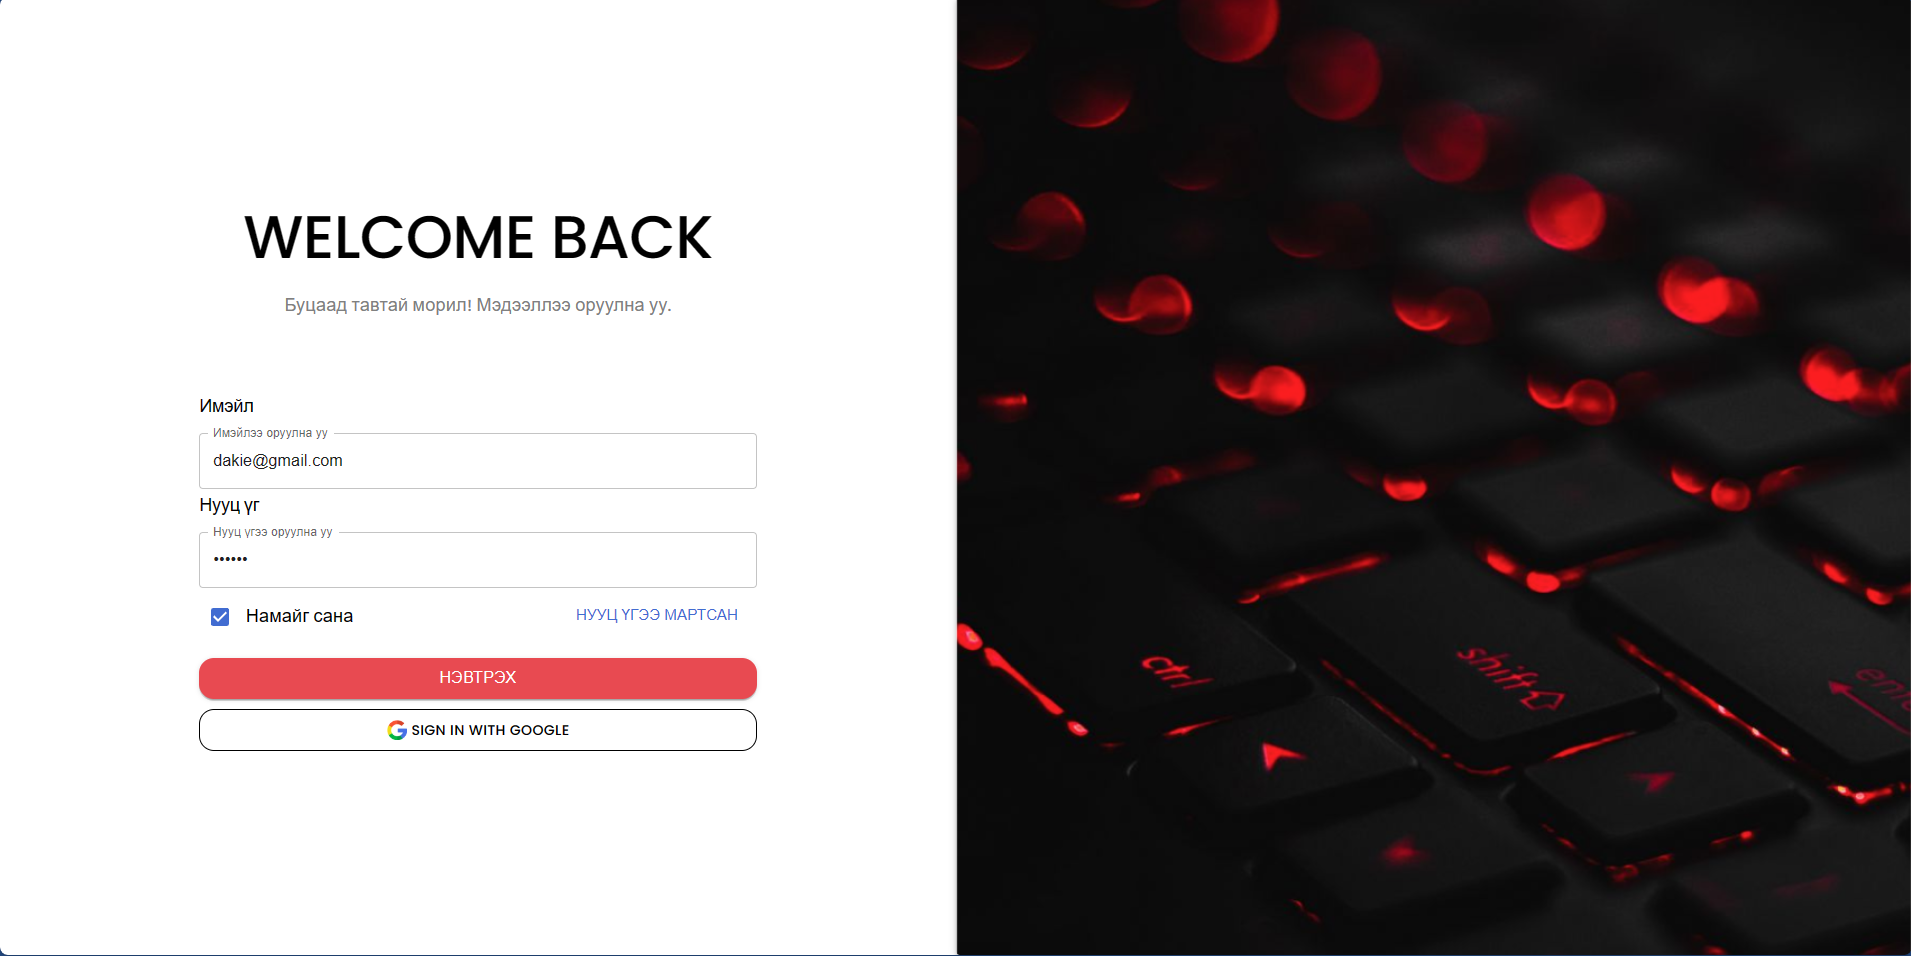
\includegraphics[width=13cm]{images/result/loginpage.png}
	\caption{Нэвтрэх хуудас}
	\label{fig:results}
\end{figure}